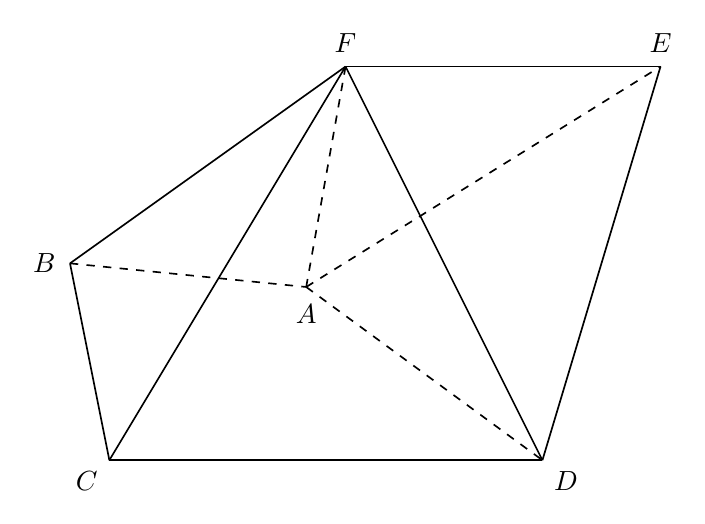
\begin{tikzpicture}[x=1cm,y=1cm,font=\normalsize,
  edge/.style={draw=black,line width=.6pt},
  hid/.style={draw=black,line width=.6pt,dashed},
  lbl/.style={font=\normalsize,inner sep=2pt}]
\coordinate (F) at (3.5,5.0);
\coordinate (E) at (7.5,5.0);
\coordinate (B) at (0.0,2.5);
\coordinate (A) at (3.0,2.2);
\coordinate (C) at (0.5,0.0);
\coordinate (D) at (6.0,0.0);
% top edge
\draw[edge] (F) -- (E);
% hidden edges through A
\draw[hid] (F) -- (A);
\draw[hid] (B) -- (A);
\draw[hid] (A) -- (E);
\draw[hid] (A) -- (D);
% base and sides
\draw[edge] (B) -- (C);
\draw[edge] (C) -- (D);
\draw[edge] (E) -- (D);
% diagonals from F
\draw[edge] (F) -- (B);
\draw[edge] (F) -- (C);
\draw[edge] (F) -- (D);
% labels with clearance
\node[lbl,above=3pt] at (F) {$F$};
\node[lbl,above=3pt] at (E) {$E$};
\node[lbl,left=3pt] at (B) {$B$};
\node[lbl,below=4pt] at (A) {$A$};
\node[lbl,below left=2pt] at (C) {$C$};
\node[lbl,below right=2pt] at (D) {$D$};
\end{tikzpicture}
